\definecolor{lightblue}{rgb}{0.67,0.87,0.9}


%------------------------------------------------
\section{Motivation \& References}
%------------------------------------------------
\begin{frame}{Motivation \& References}
    Motivation: Reachability and Büchi games are important in system verification and testing. Computing the winning set of Büchi games is a central problem in computer aided verification with a large number of applications.\\~
    
    References: \\~
    \footnotesize{
        \begin{thebibliography}{99}
            \bibitem[Smith, 2012]{p1} John Smith (2012)
            \newblock Title of the publication
            \newblock \emph{Journal Name} 12(3), 45 -- 678.
        \end{thebibliography}
    }
\end{frame}
\section{Reachability Game}
\begin{frame}{Reachability Game}
    A reachability game is a 2-player (namely P0 and P1) game on a directed finite graph.\\~
    Game graph: directed graph $G(\{V_0\cup V_1\},E)$.($\{V_0,V_1\}$is a partition of $V$) \\~
    Target set: target set is $T\subseteq \{V_0\cup V_1\}$.\\~
    A play $P$ is a (finite or infinite) path in the game graph beginning at the initial vertex $s$. If $v\in V_0$, P0 moves along an outgoing edge of v. Otherwise, P1 takes the move.\\~
    Definition of winning: P0 wins if $T\cap P \neq \emptyset$, otherwise P1 wins.\\~
    Memoryless strategy: a strategy for P0 is a mapping $\alpha : V_0 \rightarrow V$ that defines how P0 should extend the current play. 
\end{frame}
%frame 5
\begin{frame}{Example for Reachability Game}
Rectangle vertices are in $V_1$, circles are in $V_0$;\\
Vertices in $T$ are red, the initial vertex $v_I$ is blue.\\~


    \begin{columns}[c] % The "c" option specifies centered vertical alignment while the "t" option is used for top vertical alignment

        \column{.45\textwidth} % Left column and width
        \begin{adjustbox}{width=\textwidth}
            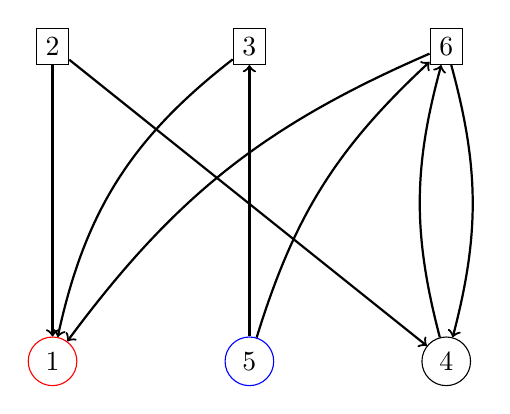
\begin{tikzpicture}
                \node[shape=circle,draw=red] (1) at (0,0) {1};
                \node[shape=rectangle,draw=black] (2) at (0,4) {2};
                \node[shape=rectangle,draw=black] (3) at (2.5,4) {3};
                \node[shape=circle,draw=black] (4) at (5,0) {4};
                \node[shape=circle,draw=blue] (5) at (2.5,0) {5};
                \node[shape=rectangle,draw=black] (6) at (5,4) {6} ;
                \path [->] (2) edge[thick] node[] {} (1);
                \path [->] (2) edge[thick] node[] {} (4);
                \path [->] (6) edge[thick,bend left=15] node[] {} (4);
                \path [->] (4) edge[thick,bend left=15] node[] {} (6);
                \path [->] (5) edge[thick,bend left=15] node[] {} (6);
                \path [->] (6) edge[thick,bend right=15] node[] {} (1);
                \path [->] (5) edge[thick] node[] {} (3);
                \path [->] (3) edge[thick,bend right=20] node[] {} (1);
            \end{tikzpicture}
        \end{adjustbox}

        \column{.5\textwidth} % Right column and width
        A winning play for P0 is $\{5,3,1\}$\\~
    \end{columns}
\end{frame}

%frame 6
\begin{frame}{Algorithm for Reachability Game}
\begin{figure}
    \centering
    \begin{adjustbox}{width=0.3\textwidth}
    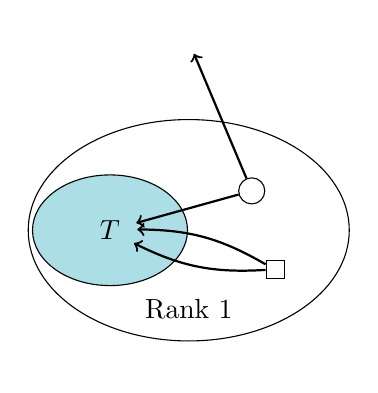
\begin{tikzpicture}
        % \draw (0,0) node {};
        \draw[fill=lightblue] (6,0) ellipse (28pt and 20pt);
        \draw[] (7,0) ellipse (58pt and 40pt);
        \node[shape=circle,draw=lightblue](t) at (6,0)  {$T$};
        \node[shape=circle,draw=white](o) at (7,2.4)  {};
        \node[shape=circle,draw=black] (1) at (7.8,0.5) {};
        \node[shape=rectangle,draw=black] (2) at (8.1,-0.5) {};
        \path [->] (1) edge[thick] node[] {} (t);
        \path [->] (1) edge[thick] node[] {} (o);
        \path [->] (2) edge[thick,bend left=15] node[] {} (t);
        \path [->] (2) edge[thick,bend right=15] node[] {} (t);
        \node[shape=circle,draw opacity=0](txt) at (7,-1)  {Rank 1};
    \end{tikzpicture}
    \end{adjustbox}
\end{figure}
    \begin{itemize}
        \item if $s$ is in $T$, P0 wins;
        \item if $s\in V_0$ and $s$ has at least one outgoing edge to $u\in T$, P0 wins in one step;
        \item if $s\in V_1$ and all of $s$'s outgoing edges go to $u\in T$, P0 wins in one step;
    \end{itemize}
\end{frame}
%frame 7
\begin{frame}{Algorithm for Reachability Game}
    We defined Rank 0 and Rank 1 already, now we define Rank i.\\
    
    $R_i:=\{v\in V|$ P0 can force a visit from v to a vertex in $T$ in i steps$\}$\\~
    
    Define Reachability set of $T$ for P0, $Reach(T,0) := \bigcup_{i=1}^{n-1}R_i$\\~
    
    
        A vertex $v\in R_i$: \\~
            if $v \in V_0$ and there is an edge $e(v,u)\quad u\in R_{i-1}$;\\~
            if $v \in V_1$ and for every edge $e(v,u)$ we have $u\in \bigcup_{j=0}^{i-1} R_j$;\\
        
\end{frame}
%frame 8
\begin{frame}{Algorithm for Reachability Game}
     \begin{columns}[c] % The "c" option specifies centered vertical alignment while the "t" option is used for top vertical alignment
    \column{.35\textwidth} % Left column and width
    \begin{adjustbox}{width=\textwidth}
    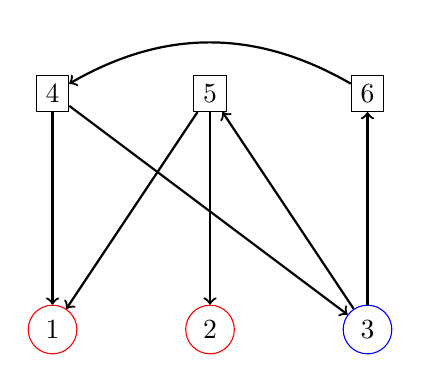
\begin{tikzpicture}
    \node[shape=circle,draw=red] (1) at (0,0) {1};
    \node[shape=circle,draw=red] (2) at (2,0) {2};
    \node[shape=circle,draw=blue] (3) at (4,0) {3};
    \node[shape=rectangle,draw=black] (4) at (0,3) {4};
    \node[shape=rectangle,draw=black] (5) at (2,3) {5};
    \node[shape=rectangle,draw=black] (6) at (4,3) {6} ;
    \path [->] (3) edge[thick] node[] {} (6);
    \path [->] (3) edge[thick] node[] {} (5);
    \path [->] (5) edge[thick] node[] {} (1);
    \path [->] (5) edge[thick] node[] {} (2);
    \path [->] (4) edge[thick] node[] {} (1);
    \path [->] (4) edge[thick] node[] {} (3);
    \path [->] (6) edge[thick, bend right=30] node[] {} (4);
    \end{tikzpicture}
    \end{adjustbox}

    \column{.6\textwidth} % Right column and width
    
             \begin{itemize}
                \item $R_0=\{1,2\}$;
                \item $R_1=\{5\}$;
                \item $R_2=\{3\}$;
                \item $R_3=\{4\}$;
                \item $R_4=\{6\}$;
            \end{itemize}
            For simplicity, denote $u\in R_k$ by Rank[$u$]=k.
    \end{columns}
\end{frame}
% frame 9
\begin{frame}{An O(m) Algorithm for Reachability Game}
    \begin{algorithm}[H]
        \scriptsize
        \SetAlgoLined
        \KwData{game graph $G$, target set $T$}
        \KwResult{Rank[$|V|$]}
        Q:= an empty queue\;
        Rank[$|V|$],count[$|V|$]:= all 0s array\;
        Q.push({T})\;
        \While{Q is not empty}{
            $u$:=Q.front,Q.pop\;
            \For{$e(v,u)\in E$}{
                \uIf{$v\in V_0$ and $v$ has not been visited}
                    {Rank[$v$]:=Rank[$u$]+1; Q.push($\{v\}$)}
                \ElseIf{$v\in V_1$}{
                    count[v]:=count[v]+1\;
                    \lIf{count[v]=Out Degree of $v$}{
                        Rank[$v$]:=Rank[$u$]+1; Q.push($\{v\}$)
                    }
                }
            }
        }
        
        \caption{Reachability for P0}
    \end{algorithm}
    Every edge is used at most once.
\end{frame}
%frame 10
\begin{frame}{Type}
    $T_1,T_2,...,T_k$ are disjoint subsets of $V$, now we want to compute Reachability of each one of them.\\~\\


    \begin{columns}
    \column{.45\textwidth} % Left column and width
    \begin{adjustbox}{width=\textwidth}
    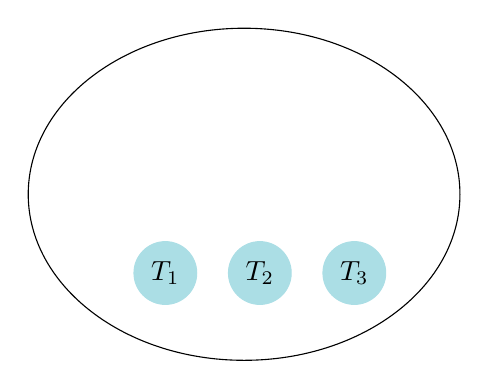
\begin{tikzpicture}
        \draw (0,0) node {};
        %\draw[fill=lightblue] (1,0) ellipse (28pt and 20pt);
        \draw[] (2,1) ellipse (78pt and 60pt);
        \node[shape=circle,draw=lightblue,fill =lightblue](t) at (1,0)  {$T_1$};
        \node[shape=circle,draw=lightblue,fill =lightblue](t) at (2.2,0)  {$T_2$};
        \node[shape=circle,draw=lightblue,fill =lightblue](t) at (3.4,0)  {$T_3$};
       % \node[shape=circle,draw=white](o) at (2,2.4)  {};
        %\node[shape=circle,draw=black] (1) at (2.8,0.5) {};
       % \node[shape=rectangle,draw=black] (2) at (3.1,-0.5) {};
       
    \end{tikzpicture}
    \end{adjustbox}

    \column{.5\textwidth} % Right column and width
        \textbf{Definition} A type of vertex $x$ is a tuple $(y_1, \ldots, y_k)$, where each $x_i \in \{0,1\}$, such that $y_i=1$ iff $x$ is in $Reach (T_i, 0)$.
    \end{columns}
\end{frame}
%frame 11
\begin{frame}{Compute Types}
    \begin{itemize}
        \item Run reachability algorithm for every $T_i$, $O(km)$;
        \item Compute simultaneously.
%        \begin{itemize}
%            \item similar to Algorithm 1, updating Ranks is replaced with updating Types.
%            \item one update needs $O(k)$, $O(m)$ times of update is needed. $O(km)$
%        \end{itemize}
        \item Can it be done in linear or nearly linear time?
    \end{itemize}
\end{frame}
%frame 12
\begin{frame}{Minimum Base}
    The minimum base of $T$ is the minimum subset of $T$ which can generate the same Reachability set as $T$.\\~
    
    Computing the minimum base is NP-hard.\\~
    
    Set cover problem: Given a set $S$ of n elements, a collections $S_1,S_2,...,S_m$ of subsets of $S$, and a number K, does there exists a collection of at most k of these sets whose union is equal to all of $S$.
    
\end{frame}
%frame 13
\begin{frame}{Minimum Base}
    \textbf{Proof}:\\
    We prove that the decision problem for minimum base is NP-Complete.\\
    The decision problem $L$ is can we find a base with at most k vertices.\\
    \begin{enumerate}
        \item $L$ is in NP.
        \item set cover problem(which is NP-Complete) can be reduced to $L$ in polynomial time.
        \begin{itemize}
            \item Construct a Reachability game graph $G(V_0,E)$. There are $m$ vertices in $T$ representing $m$ subsets in set cover problem, $n$ vertices not in $T$ representing $n$ elements in $S$.
            \item If subset $S_i$ contains element $x_j$, connect an edge from vertex representing $S_i$ to vertex representing $x_j$ in $T$.
        \end{itemize}
    \end{enumerate}
    %So $L$ is NP-Complete. The minimum base problem is NP-Hard.
\end{frame}
\begin{frame}{Minimum Base}
    \begin{adjustbox}{width=\textwidth}
    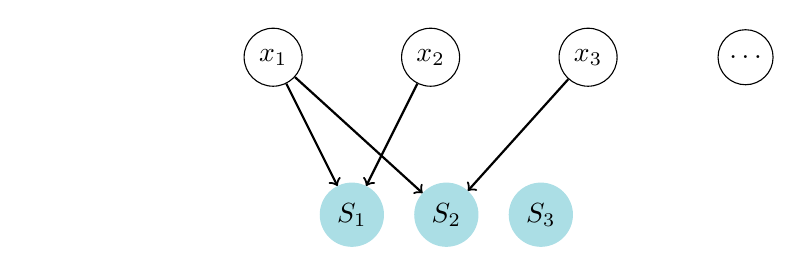
\begin{tikzpicture}
        \draw (0,0) node {};
        \node[shape=circle,draw=lightblue,fill =lightblue](t1) at (4,0)  {$S_1$};
        \node[shape=circle,draw=lightblue,fill =lightblue](t2) at (5.2,0)  {$S_2$};
        \node[shape=circle,draw=lightblue,fill =lightblue](t3) at (6.4,0)  {$S_3$};
        \node[shape=circle,draw=black](x1) at (3,2) {$x_1$};
        \node[shape=circle,draw=black](x2) at (5,2) {$x_2$};
        \node[shape=circle,draw=black](x3) at (7,2) {$x_3$};
        \node[shape=circle,draw=black](x4) at (9,2) {$\ldots$};
        \path [->] (x1) edge[thick] node[] {} (t1);
        \path [->] (x2) edge[thick] node[] {} (t1);
        \path [->] (x1) edge[thick] node[] {} (t2);
        \path [->] (x3) edge[thick] node[] {} (t2);
    \end{tikzpicture}
    \end{adjustbox}\\
    
        $S_1=\{x_1,x_2\}$\\
        $S_2=\{x_1,x_3\}$\\~
    
    So $L$ is NP-Complete. The minimum base problem is NP-Hard.
\end{frame}

\section{Büchi Game}
%frame 14
\begin{frame}{Büchi Game}
    \textbf{Definition} A \textbf{Büchi game} is a game $\mathcal{G}=(G,s,T)$ where $G$ is the Reachability game graph, $V_i$ is an initial vertex, $T\subseteq V$ is the target set as in Reachability game.\\~
    Play: The definition of play in Büchi Game is the same as in Reachability game.\\~
    Definition of winning: We assume the play $P$ is infinite here.
        if there exists infinite many vertices $v\in T$ in $P$, P0 wins. Otherwise P1 wins.

\end{frame}
%frame 15
\begin{frame}{Example for Büchi Game}
    \begin{columns}
    \column{0.45\textwidth}
    \begin{adjustbox}{width=\textwidth}
        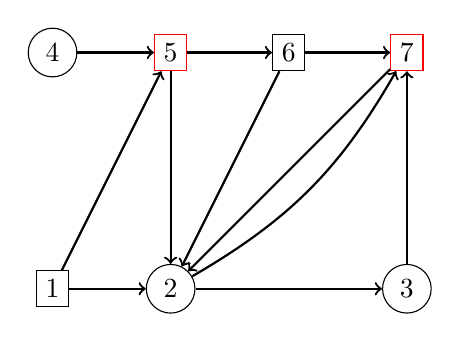
\begin{tikzpicture}
        \node[shape=rectangle,draw=black] (1) at (0,0) {1};
        \node[shape=circle,draw=black] (2) at (1.5,0) {2};
        \node[shape=circle,draw=black] (3) at (4.5,0) {3};
        \node[shape=circle,draw=black] (4) at (0,3) {4};
        \node[shape=rectangle,draw=red] (5) at (1.5,3) {5};
        \node[shape=rectangle,draw=black] (6) at (3,3) {6} ;
        \node[shape=rectangle,draw=red] (7) at (4.5,3) {7} ;
        \path [->] (4) edge[thick] node[] {} (5);
        \path [->] (5) edge[thick] node[] {} (6);
        \path [->] (6) edge[thick] node[] {} (7);
        \path [->] (3) edge[thick] node[] {} (7);
        \path [->] (2) edge[thick] node[] {} (3);
        \path [->] (1) edge[thick] node[] {} (2);
        \path [->] (1) edge[thick] node[] {} (5);
        \path [->] (5) edge[thick] node[] {} (2);
        \path [->] (6) edge[thick] node[] {} (2);
        \path [->] (7) edge[thick] node[] {} (2);
        \path [->] (2) edge[thick,bend right=15] node[] {} (7);
        
        \end{tikzpicture}
    \end{adjustbox}
    \column{0.5\textwidth}
       % P0 can force a visit from any vertex in $S=\{2,3,5,6,7\}$ to any other vertex in $S$.\\~
        
        P0 is always winning on this game graph.
    \end{columns}
\end{frame}
\begin{frame}{Algorithm for Büchi Game 1}
    \begin{columns}[c] % The "c" option specifies centered vertical alignment while the "t" option is used for top vertical alignment
    \column{.6\textwidth} % Left column and width
    \begin{adjustbox}{width=\textwidth}
    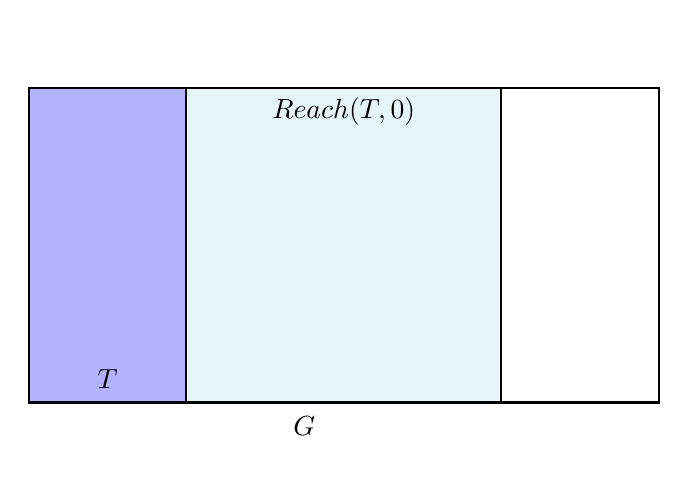
\begin{tikzpicture}
        \draw[thick, fill opacity=0.3] (0,-2) -- (0,2) -- (8,2) -- (8,-2) -- cycle;                 % G
        \draw[thick,fill=blue, fill opacity=0.3] (0,-2) -- (0,2) -- (2,2) -- (2,-2) -- cycle;  % T
        \draw[thick,fill=lightblue, fill opacity=0.3] (2,-2) -- (2,2) -- (6,2) -- (6,-2) -- cycle;  % reach
        \node[shape=circle,draw opacity=0](txt) at (3.5,-2.3)  {$G$};
        \node[shape=circle,draw opacity=0](txt) at (1,-1.7)  {$T$};
        \node[shape=circle,draw opacity=0](txt) at (4,1.7)  {$Reach(T,0)$};

    \end{tikzpicture}
    \end{adjustbox}

    \column{.35\textwidth} % Right column and width
        If $v\notin Reach(T,0)\cup T$, $v$ can not reach $T$, P0 will lose.\\~
        
        Some vertices in $T$ can not reach $Reach(T,0)\cup T$, P0 will also lose on these vertices.

    \end{columns}
\end{frame}
\begin{frame}{Algorithm for Büchi Game 1}
    \begin{columns}[c] % The "c" option specifies centered vertical alignment while the "t" option is used for top vertical alignment
    \column{.6\textwidth} % Left column and width
    \begin{adjustbox}{width=\textwidth}
    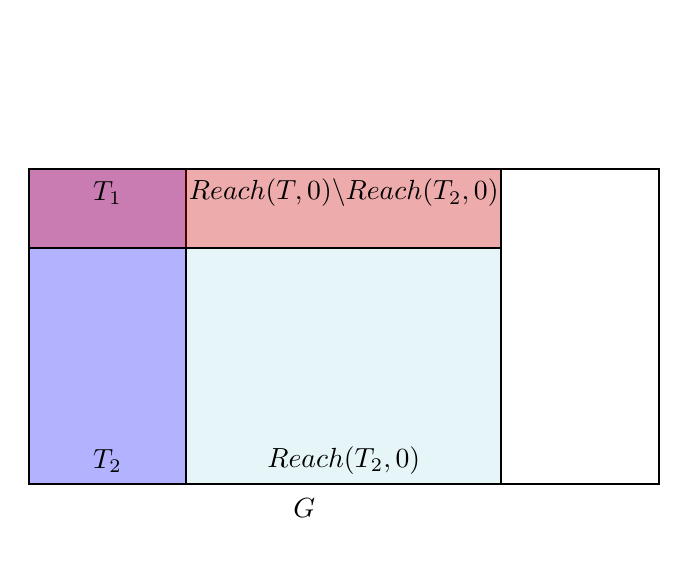
\begin{tikzpicture}
        \draw[thick, fill opacity=0.3] (0,-2) -- (0,2) -- (8,2) -- (8,-2) -- cycle;                 % G
        \draw[thick,fill=blue, fill opacity=0.3] (0,-2) -- (0,2) -- (2,2) -- (2,-2) -- cycle;  % T
        \draw[thick,fill=lightblue, fill opacity=0.3] (2,-2) -- (2,2) -- (6,2) -- (6,-2) -- cycle;  % reach
        \draw[thick,fill=red, fill opacity=0.3] (0,1) -- (0,2) -- (6,2) -- (6,1) -- cycle;  % reach
        \node[shape=circle,draw opacity=0](txt) at (3.5,-2.3)  {$G$};
        \node[shape=circle,draw opacity=0](txt) at (1,-1.7)  {$T_2$};
        \node[shape=circle,draw opacity=0](txt) at (1,1.7)  {$T_1$};
        \node[shape=circle,draw opacity=0](txt) at (4,-1.7)  {$Reach(T_2,0)$};
        \node[shape=circle,draw opacity=0](txt) at (4,1.7)  {$Reach(T,0)\backslash Reach(T_2,0)$};

    \end{tikzpicture}
    \end{adjustbox}


    \column{.37\textwidth} % Right column and width
        $T_1=\{v\in T|v$ can't reach $T\cup Reach(T,0)\}$\\~
        
        Some vertices in $T_2$ can only reach $Reach(T,0)\backslash Reach(T_2,0)$\\~
        
        We find $T_3=\{v\in T_2|v$ can't reach $T_2\cup Reach(T_2,0)\}$
    \end{columns}
\end{frame}
\begin{frame}{Algorithm for Büchi Game 1}
    \begin{columns}[c] % The "c" option specifies centered vertical alignment while the "t" option is used for top vertical alignment
    \column{.6\textwidth} % Left column and width
    \begin{adjustbox}{width=\textwidth}
    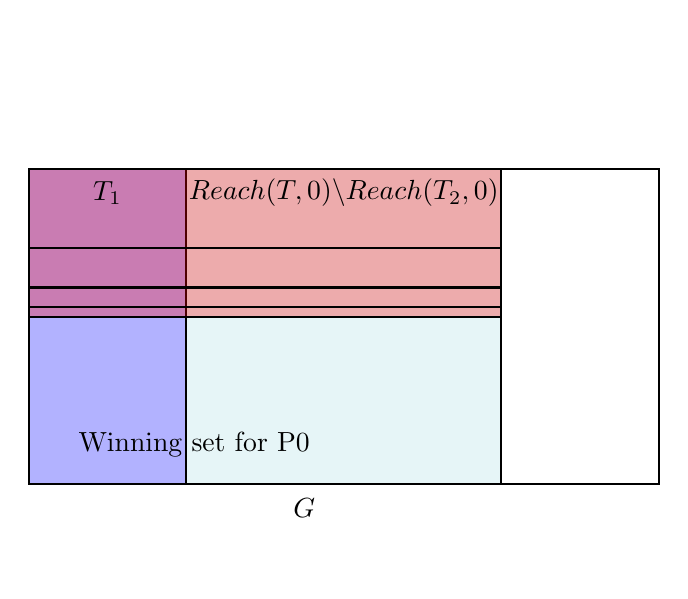
\begin{tikzpicture}
        \draw[thick, fill opacity=0.3] (0,-2) -- (0,2) -- (8,2) -- (8,-2) -- cycle;                 % G
        \draw[thick,fill=blue, fill opacity=0.3] (0,-2) -- (0,2) -- (2,2) -- (2,-2) -- cycle;  % T
        \draw[thick,fill=lightblue, fill opacity=0.3] (2,-2) -- (2,2) -- (6,2) -- (6,-2) -- cycle;  % reach
        \draw[thick,fill=red, fill opacity=0.3] (0,1) -- (0,2) -- (6,2) -- (6,1) -- cycle;
        \draw[thick,fill=red, fill opacity=0.3] (0,0.5) -- (0,1) -- (6,1) -- (6,0.5) -- cycle;
        \draw[thick,fill=red, fill opacity=0.3] (0,0.25) -- (0,0.5) -- (6,0.5) -- (6,0.25) -- cycle;
        \draw[thick,fill=red, fill opacity=0.3] (0,0.125) -- (0,0.25) -- (6,0.25) -- (6,0.125) -- cycle;
        \node[shape=circle,draw opacity=0](txt) at (3.5,-2.3)  {$G$};
        \node[shape=circle,draw opacity=0](txt) at (1,1.7)  {$T_1$};
        \node[shape=circle,draw opacity=0](txt) at (4,1.7)  {$Reach(T,0)\backslash Reach(T_2,0)$};
        \node[shape=circle,draw opacity=0](txt) at (2.1,-1.5)  {Winning set for P0};

    \end{tikzpicture}
    \end{adjustbox}

    \column{.35\textwidth} % Right column and width
        We repeat this process until $T_k$ does not shrink.\\~
        
        The remaining part of $T_k\cup Reach(T_k,0)$ is the winning set for P0.
    \end{columns}
\end{frame}
\begin{frame}{Algorithm for Büchi Game 1}
    \begin{itemize}
        \item How to find $T_1$\\
        
        $T_1=\{v\in T|v$ can't reach $T\cup Reach(T,0)\}$\\
        $T_1=\{v\in T|v$ can only reach $V\backslash \{T\cup Reach(T,0)\}\}$\\
        P1 wants to reach $V\backslash \{T\cup Reach(T,0)\}\}$, P0 tries to avoid $V\backslash \{T\cup Reach(T,0)\}\}$.\\
        compute $Reach(V\backslash \{T\cup Reach(T,0)\}\},1)$
        
        \item Time complexity\\
            $O(m)$ to find $T_i$, at most $O(n)$ times. Worst-case $O(nm)$.
    \end{itemize}
\end{frame}

\begin{frame}{Algorithm for Büchi Game 2}
    \begin{columns}[c] % The "c" option specifies centered vertical alignment while the "t" option is used for top vertical alignment
    \column{.6\textwidth} % Left column and width
    \begin{adjustbox}{width=\textwidth}
    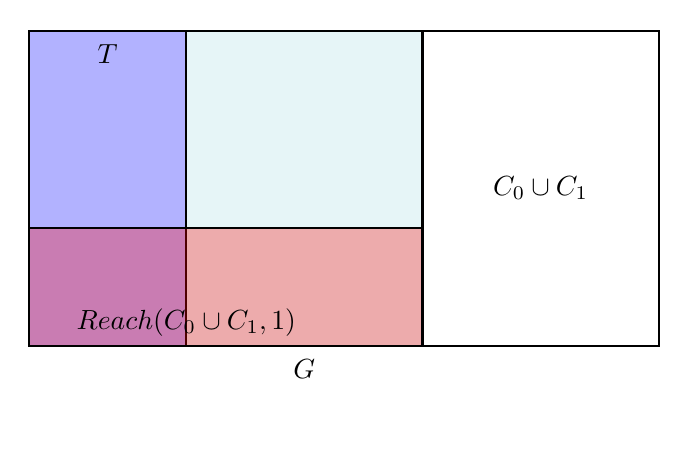
\begin{tikzpicture}
        \draw[thick, fill opacity=0.3] (0,-2) -- (0,2) -- (8,2) -- (8,-2) -- cycle;                 % G
        \draw[thick,fill=blue, fill opacity=0.3] (0,-2) -- (0,2) -- (2,2) -- (2,-2) -- cycle;  % T
        \draw[thick,fill=lightblue, fill opacity=0.3] (2,-2) -- (2,2) -- (5,2) -- (5,-2) -- cycle;  % reach
        \draw[thick,fill=red, fill opacity=0.3] (0,-2) -- (0,-0.5) -- (5,-0.5) -- (5,-2) -- cycle;  % reach
        \node[shape=circle,draw opacity=0](txt) at (3.5,-2.3)  {$G$};
        \node[shape=circle,draw opacity=0](txt) at (1,1.7)  {$T$};
        \node[shape=circle,draw opacity=0](txt) at (6.5,0)  {$C_0\cup C_1$};
        \node[shape=circle,draw opacity=0](txt) at (2,-1.7)  {$Reach(C_0\cup C_1,1)$};
        
    \end{tikzpicture}
    \end{adjustbox}


    \column{.35\textwidth} % Right column and width
        Compute $C_0$ and $C_1$.\\~
        
        $C_0$ is a set of vertices in $V_0\backslash T$ having all outgoing edges to vertices in $V\backslash T$.\\
        $C_1$ is a set of vertices in $V_1\backslash T$ having an outgoing edge to vertices in $V\backslash T$.\\~
        
        Compute $Reach(C_0\cup C_1,1)$
    \end{columns}
\end{frame}
\begin{frame}{Algorithm for Büchi Game 2}
    \begin{columns}[c] % The "c" option specifies centered vertical alignment while the "t" option is used for top vertical alignment
    \column{.6\textwidth} % Left column and width
    \begin{adjustbox}{width=\textwidth}
    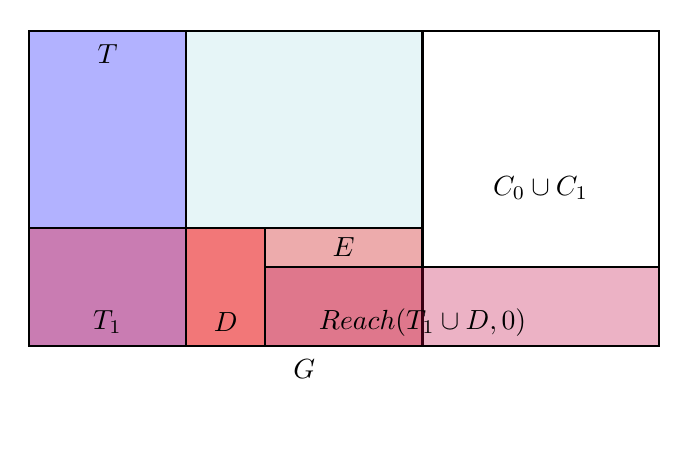
\begin{tikzpicture}
        \draw[thick, fill opacity=0.3] (0,-2) -- (0,2) -- (8,2) -- (8,-2) -- cycle;                 % G
        \draw[thick,fill=blue, fill opacity=0.3] (0,-2) -- (0,2) -- (2,2) -- (2,-2) -- cycle;  % T
        \draw[thick,fill=lightblue, fill opacity=0.3] (2,-2) -- (2,2) -- (5,2) -- (5,-2) -- cycle;  % reach
        \draw[thick,fill=red, fill opacity=0.3] (0,-2) -- (0,-0.5) -- (5,-0.5) -- (5,-2) -- cycle;  % reach
        \draw[thick,fill=red, fill opacity=0.3] (2,-2) -- (2,-0.5) -- (3,-0.5) -- (3,-2) -- cycle;  % reach
        \draw[thick,fill=purple, fill opacity=0.3] (3,-2) -- (3,-1) -- (8,-1) -- (8,-2) -- cycle;  % reach
        \node[shape=circle,draw opacity=0](txt) at (3.5,-2.3)  {$G$};
        \node[shape=circle,draw opacity=0](txt) at (1,1.7)  {$T$};
        \node[shape=circle,draw opacity=0](txt) at (6.5,0)  {$C_0\cup C_1$};
        \node[shape=circle,draw opacity=0](txt) at (1,-1.7)  {$T_1$};
        \node[shape=circle,draw opacity=0](txt) at (2.5,-1.7)  {$D$};
        \node[shape=circle,draw opacity=0](txt) at (5,-1.7)  {$Reach(T_1\cup D,0)$};
        \node[shape=circle,draw opacity=0](txt) at (4,-0.75)  {$E$};

    \end{tikzpicture}
    \end{adjustbox}

    \column{.39\textwidth} % Right column and width
    Some vertices in $Reach(C_0\cup C_1,1)$ can "reach" $T_1$.($D$ in the left picture)\\~
    
    Compute $Reach(T_1\cup D,0)$.\\~
    
    
    $E=Reach(C_0\cup C_1,1)\backslash \{T_1\cup D \cup Reach(T_1\cup D,0)\}$\\~
    
    $\{E\cup C_0\cup C_1\}\backslash Reach(T_1\cup D,0)$ is the set of vertices which can't "reach" $T$.
    \end{columns}
\end{frame}
\begin{frame}{Algorithm for Büchi Game 2}
    \begin{columns}[c] % The "c" option specifies centered vertical alignment while the "t" option is used for top vertical alignment
    \column{.6\textwidth} % Left column and width
    \begin{adjustbox}{width=\textwidth}
    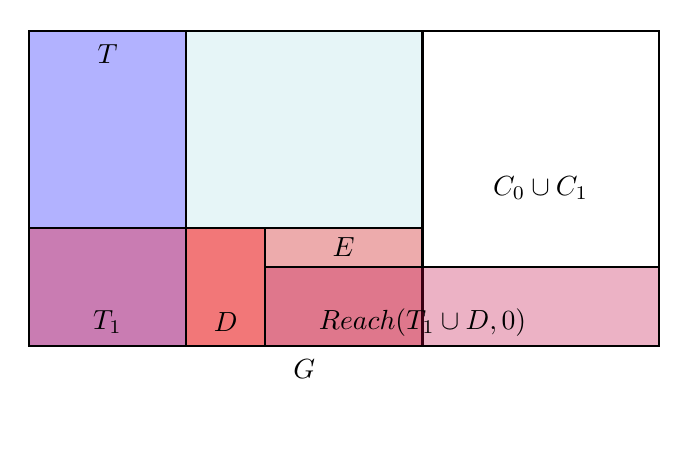
\begin{tikzpicture}
        \draw[thick, fill opacity=0.3] (0,-2) -- (0,2) -- (8,2) -- (8,-2) -- cycle;                 % G
        \draw[thick,fill=blue, fill opacity=0.3] (0,-2) -- (0,2) -- (2,2) -- (2,-2) -- cycle;  % T
        \draw[thick,fill=lightblue, fill opacity=0.3] (2,-2) -- (2,2) -- (5,2) -- (5,-2) -- cycle;  % reach
        \draw[thick,fill=red, fill opacity=0.3] (0,-2) -- (0,-0.5) -- (5,-0.5) -- (5,-2) -- cycle;  % reach
        \draw[thick,fill=red, fill opacity=0.3] (2,-2) -- (2,-0.5) -- (3,-0.5) -- (3,-2) -- cycle;  % reach
        \draw[thick,fill=purple, fill opacity=0.3] (3,-2) -- (3,-1) -- (8,-1) -- (8,-2) -- cycle;  % reach
        \node[shape=circle,draw opacity=0](txt) at (3.5,-2.3)  {$G$};
        \node[shape=circle,draw opacity=0](txt) at (1,1.7)  {$T$};
        \node[shape=circle,draw opacity=0](txt) at (6.5,0)  {$C_0\cup C_1$};
        \node[shape=circle,draw opacity=0](txt) at (1,-1.7)  {$T_1$};
        \node[shape=circle,draw opacity=0](txt) at (2.5,-1.7)  {$D$};
        \node[shape=circle,draw opacity=0](txt) at (5,-1.7)  {$Reach(T_1\cup D,0)$};
        \node[shape=circle,draw opacity=0](txt) at (4,-0.75)  {$E$};

    \end{tikzpicture}
    \end{adjustbox}

    \column{.4\textwidth} % Right column and width
    $S=\{E\cup C_0\cup C_1\}\backslash Reach(T_1\cup D,0)$ is the same as $V\backslash \{T\cup Reach(T)\}$ in Algorithm 1.\\~
    
    Then we can compute $Reach(S,1)$ to delete some losing vertices for P0 in $T$.\\~
    
    Repeat the same process on $G\backslash\{T\backslash Reach(S,1)\}$
    \end{columns}
\end{frame}
\begin{frame}{Algorithm for Büchi Game 2}
    \begin{itemize}
        \item Time complexity\\~
        
        Finding $S$ needs $O(m)$ time.\\
        Also in the worst case we need to compute $S$  $O(n)$ times. worst case $O(nm)$.
    \end{itemize}
\end{frame}
%------------------------------------------------
